\chapter{Prototyping in Office Message System}

\section{System description}
The system involves subscribers, publishers and different topics, as to show the workings of the connext middleware. 

\begin{center}
	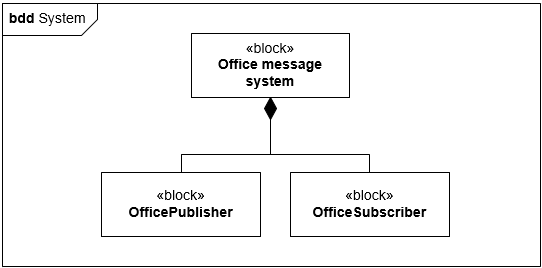
\includegraphics[width=\textwidth]{bdd_image.png}
	\captionof{figure}{BDD of the Office Message System}
\end{center}

The office message system is shown in figure 4.1. The system consists of two different classes, the OfficePublisher and the OfficeSubscriber. The specific topic, type and Quality Of Service of the Subscribers/Publishers are determined through constructor injection.

The prototype will consist of two programs running side by side. One will spawn the subscribers and the other will spawn the publishers. All Readers and Writers are configured for sending messages by the string type. 

The configuration is setup as seen in figure 4.2.

\begin{center}
	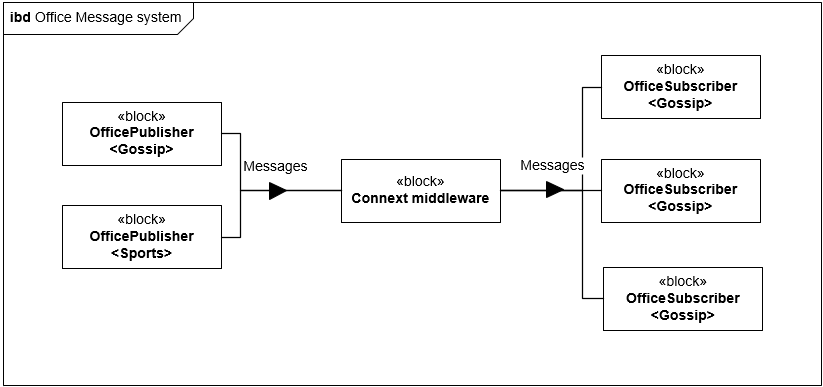
\includegraphics[width=\textwidth]{ibd_image.png}
	\captionof{figure}{IBD of the Office Message System}
\end{center}

As is seen, a publisher publishing on the "Gossip" topic and one for the "Sports" topic are in the system. The publishers will communicate to the subscribers through the connext middleware.

\subsection{OfficePublisher}
This class is used as a wrapper, containing most of the RTI classes. This is not to be confused with the RTI Publisher class. 

The constructor for this class takes references to the needed QoS's as arguments. It also takes a String with the name of the topic, the DataWriter should publish to. This way, an OfficePublisher can be configured to publish to an arbitrary Topic (We use "Gossip" and "Sport"). The difference between the publishers, is then merely the topics they publish to.

The OfficePublisher has a public method \textit{PublishMessage(String message)}. When invoked, this message publishes the message to the middleware with the OfficePublishers topic. 

\subsection{OfficeSubscriber}
This class is used as a wrapper, containing most of the RTI classes needed for creating a subscriber. This is not to be confused with the RTI Subscriber class.

The constructor for this class takes references to the needed QoS's as arguments. It also takes a String with the name of the topic, the DataReader should subscribe to. This way, an OfficeSubscriber can be configured to subscribe to an arbitrary Topic (We use "Gossip" and "Sport"). The difference between the subscrubers, is then merely the topics they publish to.

The OfficeSubscriber extends the class \textit{DataReaderAdapter}. This way, an object of this class can pass a pointer to itself as a listener-object on the DataReader (see DataReader section).

\section{Connext RTI}
The Connext RTI middle ware implementation gives access to a series of objects and implementations for communicating over the network.

The functionality is implemented in lower level languages and is exposed through several high-level languages (C\#, Java etc.). Our prototype is written in Java, as we wanted to run the prototype on Linux. 

To use the functionality of Connext (e.g. interconnecting publishers and subscribers), the right classes must be used. The classes used, will be described in the following. 

\subsection{Domain Participant}
The Domain Participant is the main interface to the domain (see section 2.6). This class enables us to create all the other classes needed for communication through the middleware.

This class makes sure that all other created classes are created for the correct domain. This is created with an injected QoS object (set to default).

\begin{center}
	\fbox{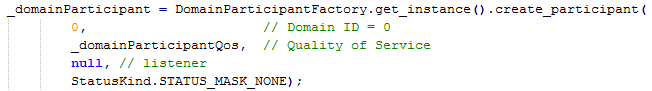
\includegraphics[width=\textwidth]{creatingDomainParticipant.png}}
	\captionof{figure}{Creating the DomainParticipant in OfficePublisher constructor}
\end{center}

\subsection{Topics}
Our subscription model is Topic based, meaning that the middleware only distinguishes between messages based on the topic they were created for. 

The topic is created through a Factory Method exposed by the created domain participant. The name and data type of the topic will be given as arguments to this method. 

The topic name is the string, identifying the topic on the domain. This is the identifier for the topic. 

The Topic type is the type of data, that will be transferred for the topic. This could be used to make two topics with the same name disticnt from each other, based on the type of data.
Our topics are using the built-in string type to transfer messages.
Custom types can be implemented as IDL.

When creating custom types, it is possible to designate one of the fields in the type as a \textit{Key}. Subscribers can then filter on the key and thus, not receive all data published on the topic they subscribed to.

\begin{center}
	\fbox{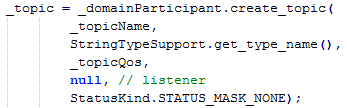
\includegraphics[scale=1]{creatingTopic.png}}
	\captionof{figure}{Creating the Topic in OfficePublisher constructor}
\end{center}


\section{Publisher}
To publish data on the domain, a publisher and a DataWriter are needed. The Publisher is used for control of the DataWriter. 
A DataWriter can only write to one specific Topic. A Publisher object can be used for grouping an arbitrary number of DataWriters with an overall QoS and specific settings.
In this application, this grouping is not needed, so a Publisher object is not created explicitly. The middleware will use a default Publisher, hidden from the user.

\subsection{DataWriter}
This object takes care of the actual writing to the domain. A specific implementation of the object, StringDataWriter is used to publish messages with the String type. 

As we do not have a specific Publisher, the DataWriter is created through the DomainParticipant with the created Topic object as argument.

\begin{center}
	\fbox{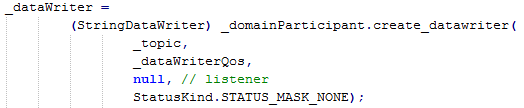
\includegraphics[scale=1]{creatingDataWriter.png}}
	\captionof{figure}{Creating the StringDataWriter in OfficePublisher constructor.}
\end{center}

The writer exposes a \textit{Write(String message)} function, used for publishing data.

\section{Subscriber}
To subscribe to data on a topic, a Subscriber and a DataReader are needed. The Subscriber class can be used to group DataReaders and set common QoS parameters. Just like with the Publisher this isn't actually needed, as the middleware can implicitly create a default Subscriber for us. 

\subsection{DataReader}
The DataReader is in charge for actually being notified of data. This object subscribes to a Topic and will receive all messages published for this topic (if they are not filtered away based on content filters and/or QoS mismatches). 

The DataReader takes a Topic object as well as a listener object for its constructor. The listener object defines a callback function, which will be called when the DataReader receives a message.

In this application, the OfficeSubscriber inherits from DataReaderAdapter, which can be passed as a listener. Thus, a pointer to the calling OfficeSubscriber is passed to the DataReader (through af \textit{this} pointer).

The reader is specifically a StringDataReader, as the topics in this system, publish Strings as messages. The StringDataReader is a builtin class in the DDS. 

 \begin{center}
	\fbox{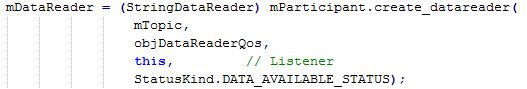
\includegraphics[scale=1]{creatingDataReader.png}}
	\captionof{figure}{Creating the StringDataReader in OfficeSubscriber constructor.}
\end{center}

The function actually reading from the DataReader is seen on the figure and is a part of the OfficeSubscriber class.

\begin{center}
	\fbox{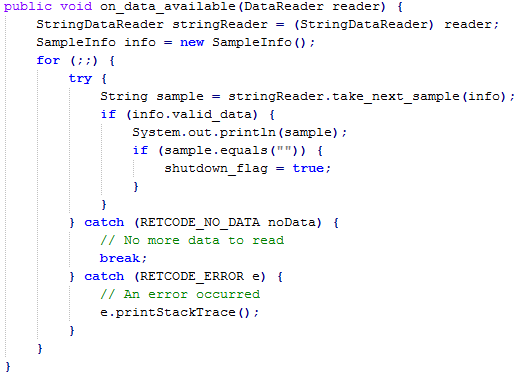
\includegraphics[scale=0.75]{on_data_available.png}}
	\captionof{figure}{The on data available function.}
\end{center}

\section{Quality Of Service}
The purpose of setting up QoS for this project, other than the defaults built in to the connect middleware, is to persist data in a way, so that a subscriber will get the last few messages, even if they were published before the subscriber became online.

We set all explicit QoS parameters programatically and inject QoS objects into the OfficePublishers and OfficeSubscribers. 

Custom QoS are set on the DataWriter and DataReader objects. QoS for DomainParticipants and Topics are set to default.

The set parameters are:

\begin{enumerate}
\item \textit{Reliability}

The reliability of the data transfer. This determines if the data is sent in a fire-and-forget manner (best effort) or if the middleware should make sure data arrives.

Set to Reliable, as we wish to make sure data arrives and the middleware must keep data to send to subscribers, subscribing at a later time.

\item \textit{Durability}

Determines if messages should be kept by the middleware and how it should be kept (persistently = on harddrive, transient = in memory).

Set to Transient, as it is not necessary to keep messages on the harddrive. We only keep 100 messages (see History) so this should not be a problem.

\item \textit{History}

Determines how many messages are kept by the middleware (if any!). This way, a new subscriber will only receive the last messages as specified by the \textit{depth} field.

Set to Keep Last History with depth 100. This makes the middleware keep the last 100 messages. 

\item \textit{Liveliness}

Determines if and how the middleware should check if DataWriters are still alive. 

Set to Automatic, to let the middleware check automatically. Lease duration set to infinite as for this system, publishers and subscribers are kept open all the time.

\end{enumerate}

\textbf{For DataWriters}
As seen on the following figure, a default QoS object is created and the custom values are then set. This is done in the main function in \textit{mainClass.java} of the publisher project and the object is then passed to the OfficePublisher constructor.
\begin{center}
	\fbox{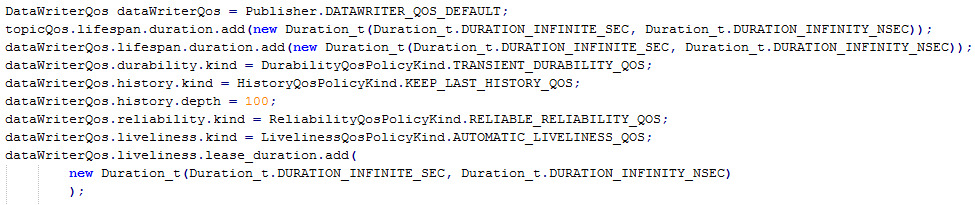
\includegraphics[width=\textwidth]{SettingQoSPublishers.png}}
	\captionof{figure}{Setting the QoS parameters programatically}
\end{center}

\textbf{For DataReaders}
As seen on the following figure, a default QoS object is created and the custom values are then set. This is done in the main function in \textit{main.java} of the subscriber project and the object is then passed to the OfficeSubscriber constructor.
\begin{center}
	\fbox{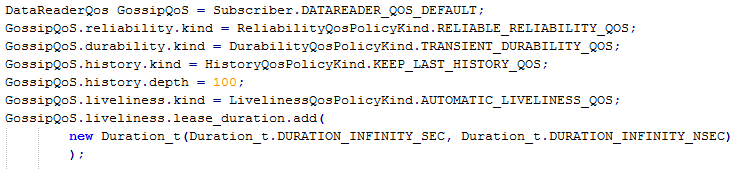
\includegraphics[width=\textwidth]{SettingQoSSubscribers.png}}
	\captionof{figure}{Setting the QoS parameters programatically}
\end{center}




\section{Tests}
For testing the created OfficeSubscriber and OfficePublishers, two small test programs are written, to set up a system as seen on figure 4.2 with two publishers (Gossip and Sport) and three Subscribers(Gossip, Sport, Sport). 

The publisher program will let a user type messages to the different topics and the subscriber program will print all incoming messages to the console.

When the program is run and messages are types into the console, to be sent, only the Sports subscriber should receive messages on the sports topic and only the Gossip subscribers should receive data published to the gossip topic. 

The main method for the publisher looks like this:

\begin{center}
	\fbox{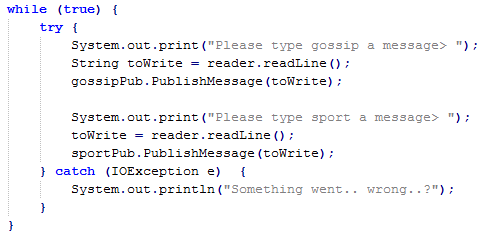
\includegraphics[scale=1]{officePubMain.png}}
	\captionof{figure}{The routine taking data from the user and publishing it to the appropriate topics.}
\end{center}

And when running the publisher main, the output is 

\begin{center}
	\fbox{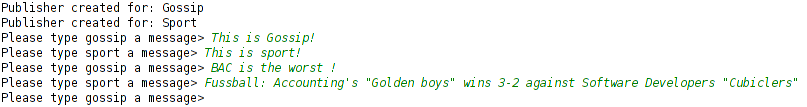
\includegraphics[scale=0.8]{outputPublisherMain.png}}
	\captionof{figure}{Output from the Publishers main. Notice the input messages.}
\end{center}

When these messages are published, the subscriber shows 

\begin{center}
	\fbox{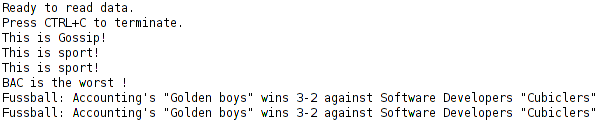
\includegraphics[scale=1]{subscriberOutputMain.png}}
	\captionof{figure}{Output from the Subscriber main. Notice the output messages.}
\end{center}

As can be seen, the input messages are shown. The Sports messages are show twice, as there are two subscribers to this.